\documentclass{article}


% load package with some of the available options - you may not need this!
\usepackage[framed,autolinebreaks,useliterate]{mcode}

% for checklist
\usepackage{enumitem,amssymb}
\newlist{todolist}{itemize}{2}
\setlist[todolist]{label=$\square$}
\usepackage{pifont}
\newcommand{\cmark}{\ding{51}}%
\newcommand{\xmark}{\ding{55}}%
\newcommand{\done}{\rlap{$\square$}{\raisebox{2pt}{\large\hspace{1pt}\cmark}}%
\hspace{-2.5pt}}
\newcommand{\wontfix}{\rlap{$\square$}{\large\hspace{1pt}\xmark}}


% something NOT relevant to the usage of the package.
\usepackage{graphicx}
\usepackage{url,textcomp}
\setlength{\parindent}{0pt}
\setlength{\parskip}{18pt}
\title{ECTA Homework 4\\Multiobjective Optimization with the\\Non-dominated Sorting Genetic Algorithm II}
\author{\color{blue}Arun Prabhu, \texttt{arun.prabhu@smail.inf.h-brs.de}\\\color{blue}Dharmin Bakaraniya, \texttt{dharmin.bakaraniya@smail.inf.h-brs.de}}
% //////////////////////////////////////////////////

\begin{document}

\maketitle

\begin{center}
	\begin{minipage}{1\linewidth}
		\begin{center}
			\includegraphics[width=\textwidth]{xkcd}
		\end{center}
	\end{minipage}
\end{center}

\newpage

\section{Assignment Description}
	\begin{enumerate}
		\item Implement the NSGA-II algorithm and apply it to a toy problem
			\begin{itemize}
			\item Bit string with length 20
			\item Maximize the number of leading zeros (zeros in a row at the front)
			\item Maximize the number of trailing ones (ones in a row at the back)
		\end{itemize}
		\item Show that your algorithm works by plotting the population at various stage of the algorithm
	\end{enumerate}

\section{Submission Instructions}
Follow along with the instructions in this PDF, filling in your own code, data, and observations as noted. Your own data should be inserted into the latex code of the PDF and recompiled. All code must be done in MATLAB.\@

To be perfectly clear we expect two submissions to LEA:\@
\begin{enumerate}
	\item 1 PDF (report) \- a modified version of your submission PDF, with your own code snippets, figures, and responses inserted
    \item 1 ZIP (code and data)   \- a \texttt{.zip} file containing all code use to run experiments (.m files) \textit{and} resulting data as a \texttt{.mat} file
	\item 1 GIF (algorithm progress) \- use the file on the MATLAB file exchange: \url{https://www.mathworks.com/matlabcentral/fileexchange/63239-gif}
\end{enumerate}


\newpage
\section{The Assignment}

\subsection{NSGA-II (75pts)}
\begin{itemize}
	\item (50pts) Implement NSGA-II to find all non-dominated solutions to the trailing ones, leading zeros problem. 
	\begin{itemize}
		\item Bitstring with length 20
		\item Population size of 100
		\item Generations 100
		\item Hints:
		\begin{itemize}
			\item Crossover and mutation can be performed just as in other bit string problems, e.g.\ one-max
			\item The \mcode{sortrows} function can be used to sort matrices, you can use this first before implementing NSGAs sorting
		\end{itemize}
        \begin{figure}[htpb]
            \centering
            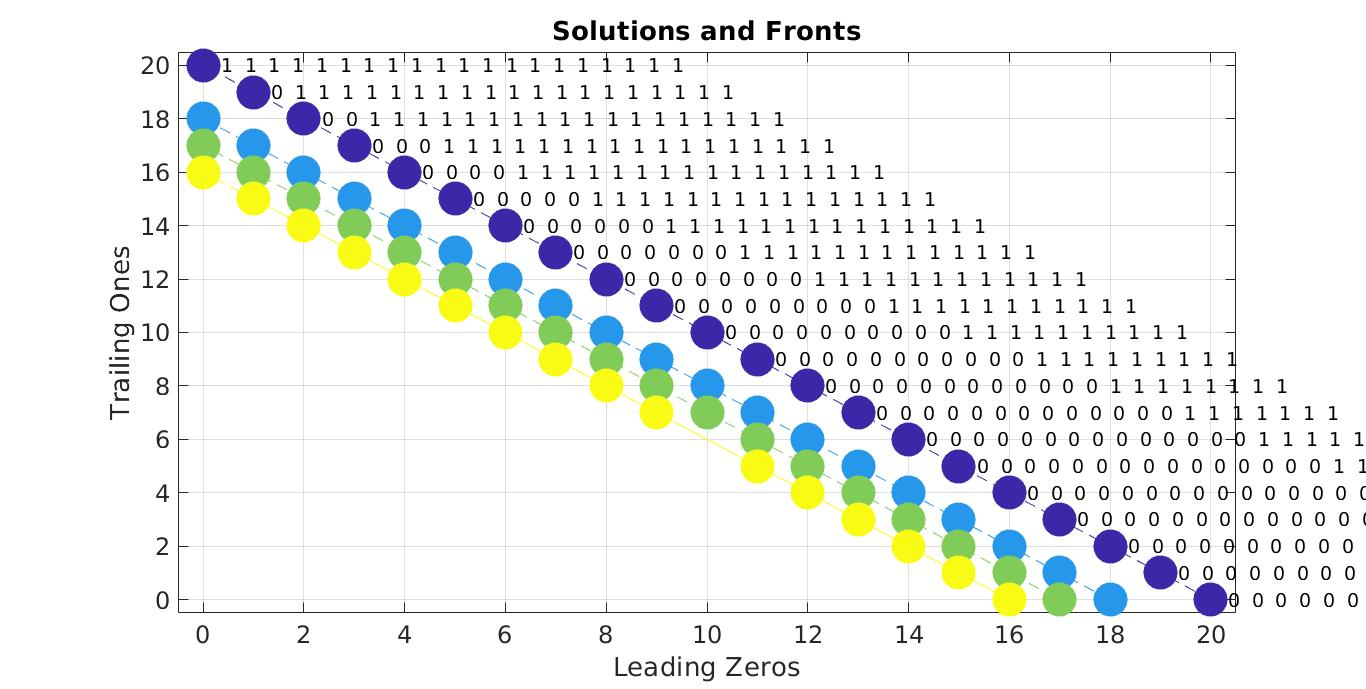
\includegraphics[width=1.0\linewidth]{section3point1_bullet1.jpg}
            \caption{Fronts of NSGA2 algorithm with 2 fitnesses (trailing ones, leading zeros) ran for 100 gen with 100 pop for bitstring of size 20.}\label{fig:}
        \end{figure}
	\end{itemize}
    \newpage
	\item (20pts) Visualize the progress of your algorithm over a single 100 generation run with an animated gif (1 frame every generation).
	\begin{itemize}
		\item Use the code here: \url{https://www.mathworks.com/matlabcentral/fileexchange/63239-gif} to create gif
		\begin{itemize}
			\item Set the timing so that the gif completes in a reasonable amount of time (between 10 and 20 seconds)
		\end{itemize}
		\item Fronts can be visualized with the code snippets attached\\ (\mcode{displayFronts.m})
	\end{itemize}
        \color{blue}
        \begin{itemize}
            \item Please refer \texttt{gif\_without\_markers.gif}
        \end{itemize}
        \color{black}
	\item (5pts) At each iteration mark the individuals which carry on to the next population, and which do not (you will have to code this yourself).
        \color{blue}
        \begin{itemize}
            \item Please refer \texttt{gif\_with\_markers.gif}
        \end{itemize}
        \color{black}
\end{itemize}

\newpage
\subsection{Short Answer (25pts)}
\begin{itemize}
	\item (10pts) Compare the sort used by NSGA-II and MATLAB's quicksort built in \mcode{sortrows} function. How long does 100 generations take with each approach when using a population size of:
        \begin{itemize}
        \color{blue}
            \item We take average of time taken over 10 experiments.
        \color{black}
        \end{itemize}
	\begin{enumerate}
		\item 10:
			\begin{itemize}
                \item Quicksort: \color{blue}0.056817 seconds\color{black}
			\item Fast non-dominated sort: \color{blue}0.082453 seconds\color{black}
			\end{itemize}
		\item 100:
			\begin{itemize}
			\item Quicksort: \color{blue}0.43277 seconds\color{black}
			\item Fast non-dominated sort: \color{blue}1.6236 seconds\color{black}
			\end{itemize}
		\item 1000:
			\begin{itemize}
			\item Quicksort: \color{blue}4.9949 seconds\color{black}
			\item Fast non-dominated sort: \color{blue}111.2765 seconds\color{black}
			\end{itemize}
	\end{enumerate}
    \begin{figure}[htpb]
        \centering
        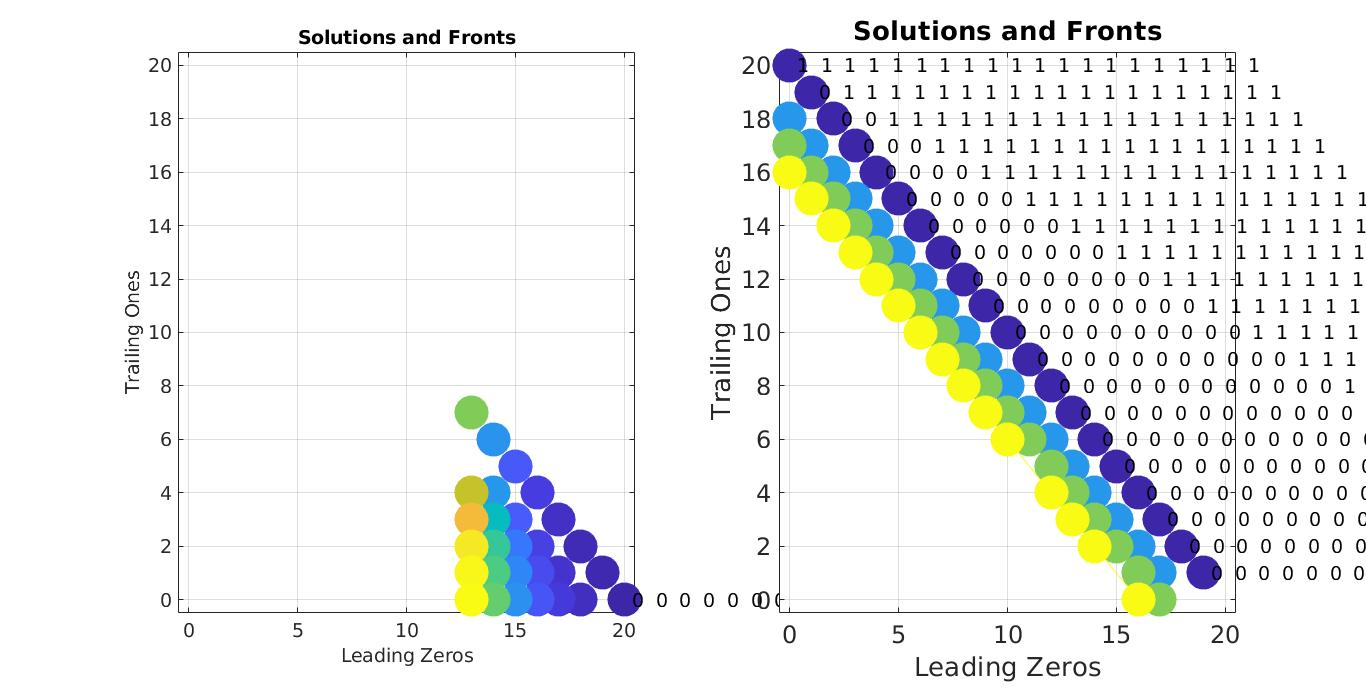
\includegraphics[width=1.0\linewidth]{section3point2_bullet1.jpg}
        \caption{Comparison of quicksort (left) with NSGA2 (right) on 2 functions (leading zeros and trailing ones) for 100 pop and 100 gen on bitstring with size 20 on a single experiment.}\label{fig:quicksortVSnsga}
    \end{figure}
    \color{blue}
    \begin{itemize}
        \item As it can be seen from Figure~\ref{fig:quicksortVSnsga}, quicksort can't even find the front because the sorting is done only with one column. Second column will only be used if first column have a tie. This implicitly gives first function (leading zeros) more importance than second function (trailing ones). This is the reason why we see that most of the population at the end is gathered at the right bottom corner.
        \item One more thing to note from Figure~\ref{fig:quicksortVSnsga} (left) is that only one individual is in first front.
        \item Because of the above reasons, we can say that eventhough quicksort takes less time compared to NSGA2, it does not find the solution and thus time should not be the only criteria of performance measurement for these algorithms.
    \end{itemize}
    \color{black}
	\item (5pts) Plot the end result of a single run with [100 pop and 100 gen] and [10 pop and 1000 gen]. Describe the difference between the end results. Which is preferable?
        \begin{figure}[htpb]
            \centering
            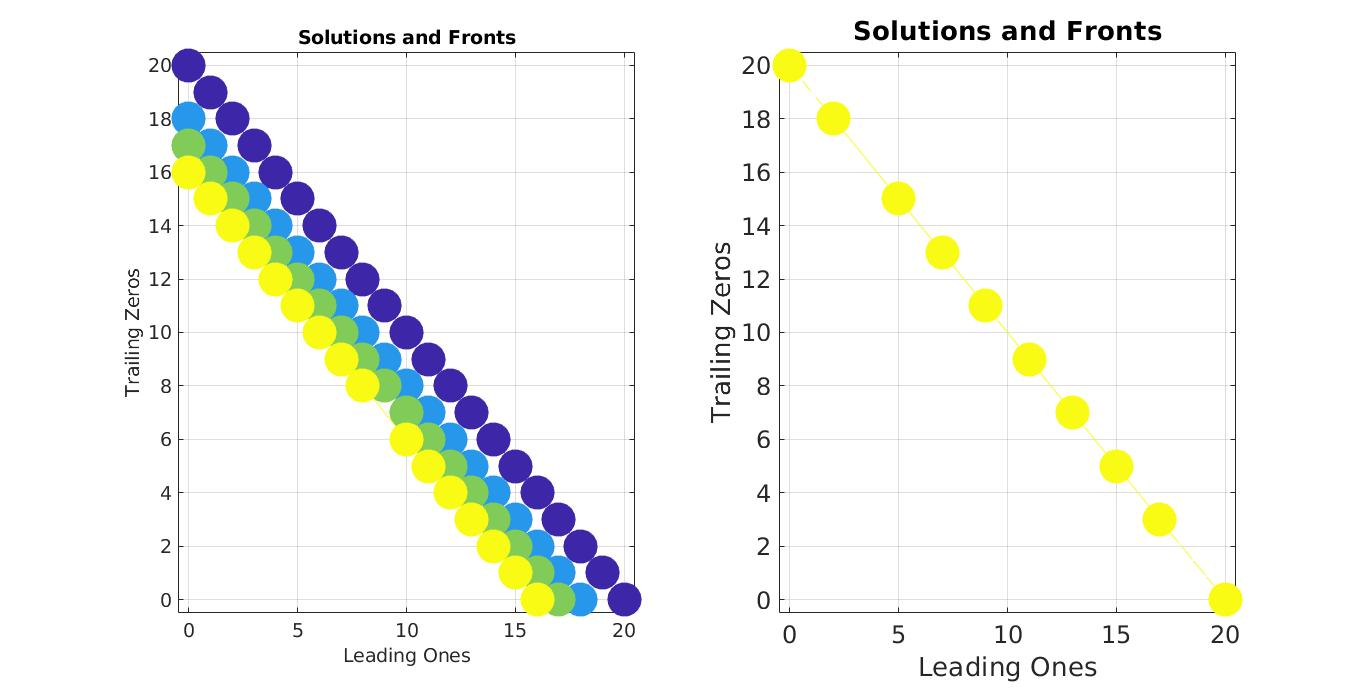
\includegraphics[width=1.0\linewidth]{section3point2_comparision.jpg}
            \caption{NSGA2 with 100 pop and 100 gen (left) VS\@. NSGA2 with 10 pop and 1000 gen (right) for solving leading zeros trailing ones problem with bitstring of length 20.}\label{fig:comparision}
        \end{figure}

        \color{blue}
        \begin{itemize}
            \item The \texttt{popSize} defines how fine grained solution is.
            \item As seen from Figure~\ref{fig:comparision}, the execution with \texttt{popSize=100} (left) produces the complete fine grained pareto front whereas the execution with \texttt{popSize=10} (right) reaches the correct pareto front but it is not able to provide the complete front because of lack of individuals.
        \end{itemize}
        \color{black}
        \newpage
	\item (5pts) Imagine you were to replace the objective of ``leading zeros'' with ``largest binary number''. Predict the result, and give your reasoning.

        \color{blue}
        \begin{itemize}
            \item We expect the first front to have only a single individual with genome of all ones. This is because maximum value of fitness function \textit{trailing ones} would be all ones which is also the maximum for function \textit{largest binary number}.
            \item Most of the individuals in any front will be odd number. This is because when the last bit is \texttt{1}, the number becomes odd.
            \item The even number in a front will occur for values for which the objective function \textit{trailing ones} is 0.
            \item As seen from Figure~\ref{fig:binary}, we can confirm our predictions mentioned above.
        \end{itemize}
        \color{black}
        \begin{figure}[htpb]
            \centering
            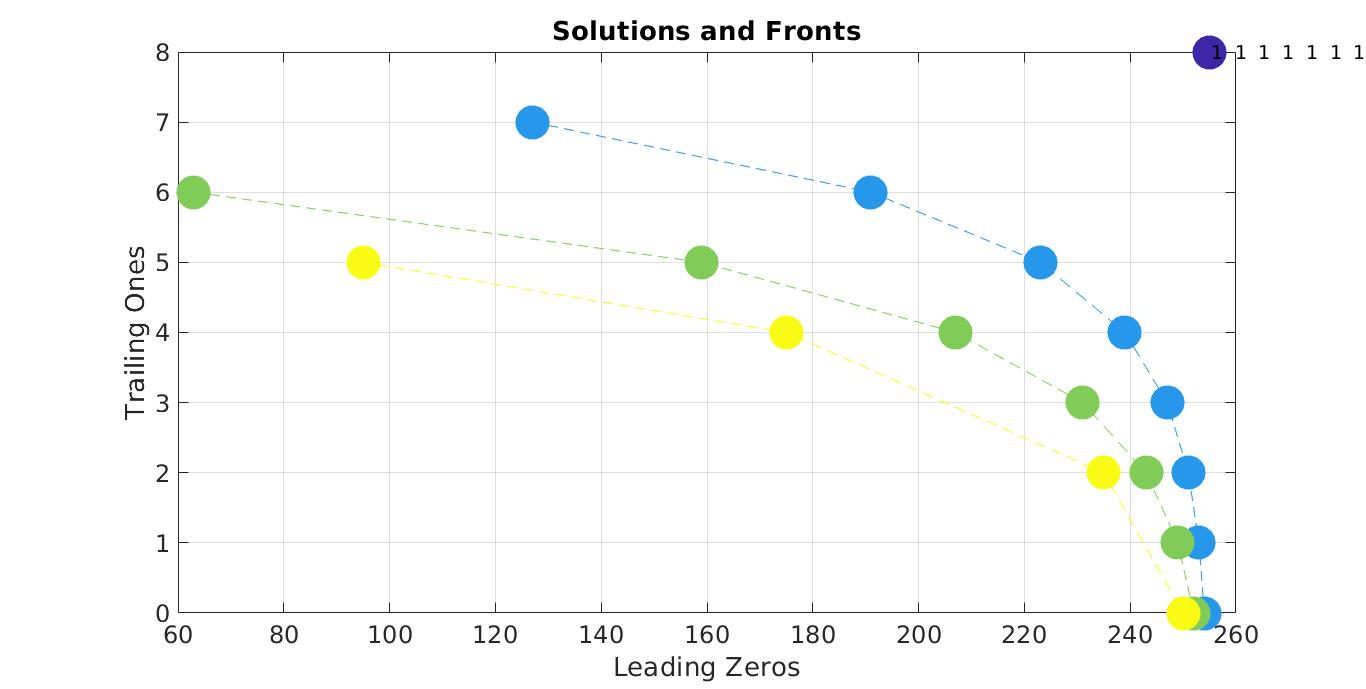
\includegraphics[width=1.0\linewidth]{section3point2_bullet3.jpg}
            \caption{NSGA2 with 20 pop and 20 gen for solving largest binary number and trailing ones problem with bitstring of length 8.}\label{fig:binary}
        \end{figure}
        \newpage
	\item (5pts) Imagine you were to add a third objective: ``non-consecutive ones and zeros'' (ones not touching ones and zeros not touching zeros, e.g. 0101 and 1010 are the most optimal 4 bit solutions). How would you adjust the hyperparameters to get a satisfactory result?
        \color{blue}
        \begin{itemize}
            \item The \texttt{popSize} has to be larger because there is an extra function. This makes the pareto front large, which in turn will need more individual to represent.
            \item The \texttt{nGeneration} must also be increased because the algorithm will require more time to find and occupy the whole pareto front.
        \end{itemize}
        \color{black}
	\item (5pts) In many GAs and ESs populations must be ranked, but no special methods are used. Why is a faster sort in MOO so important?
        \color{blue}
        \begin{itemize}
            \item We have not come across, up till now, any GAs or ESs which required sorting.
            \item Because most of the GAs and ESs have single objective function to optimize, when a sorting is required, a conventional sorting is enough, but MOO has multiple objective functions, so when they are sorted, typical sorting algorithms provide biased output (as it is seen from Figure~\ref{fig:quicksortVSnsga})
        \end{itemize}
        \color{black}
\end{itemize}

\newpage
\subsection{** Extra Credit ** (+ 10pts in examination)}
Implement the third objective ``non-consecutive ones and zeros''
\begin{enumerate}
	\item How many non-dominated solutions are possible? (Hint: start with a smaller length and test)
        \begin{table}[htpb]
            \centering
            \caption{Size of non dominated front for different genes}\label{tab:genesVSsize}
            \begin{tabular}{c|c|c}
                \textbf{nGenes (n)} & \textbf{size of front 1 (S)} & \textbf{offset (O)} \\\hline
                    2 &  3 & 5\\
                    4 &  8 & 7\\
                    6 & 15 & 9\\
                    8 & 24 & 11\\
                    10 &35 & 13\\
            \end{tabular}
        \end{table}
        \color{blue}
        \begin{itemize}
            \item $S_{n+2} = S_{n} + O_{n}$ and $O_{n+2} = O_{n} + 2$
            \item From the trends seen in Table~\ref{tab:genesVSsize}, we predict that the size of the non dominated front solution will be 120  (offset=21) for gene size of 20
        \end{itemize}
        \color{black}
	\item What changes did you make to the algorithm and hyperparameters to get a good result?
        \color{blue}
        \begin{itemize}
            \item We had to change the fitness calculation function and domination calculation functions. Plotting function was also updated to plot 3D plots.
            \item We increased the \texttt{popSize} from 100 to 150. We also increased the \texttt{nGeneration} to 200 from 100.
        \end{itemize}
        \color{black}
	\item List the solutions in your 1st front. Are they all Pareto optimal? How complete is your front (in percentage, based on $\#1$)
        \color{blue}
        \begin{itemize}
            \item Please find the solution in \texttt{extraSolution.mat}.
            \item We have 120 individuals in first front. 
            \item From our calculations above, our front is 100\% complete.
        \end{itemize}
        \color{black}
	\item Plot the end result in 3D. (Use \mcode{plot3} or \mcode{scatter3})
        \begin{figure}[htpb]
            \centering
            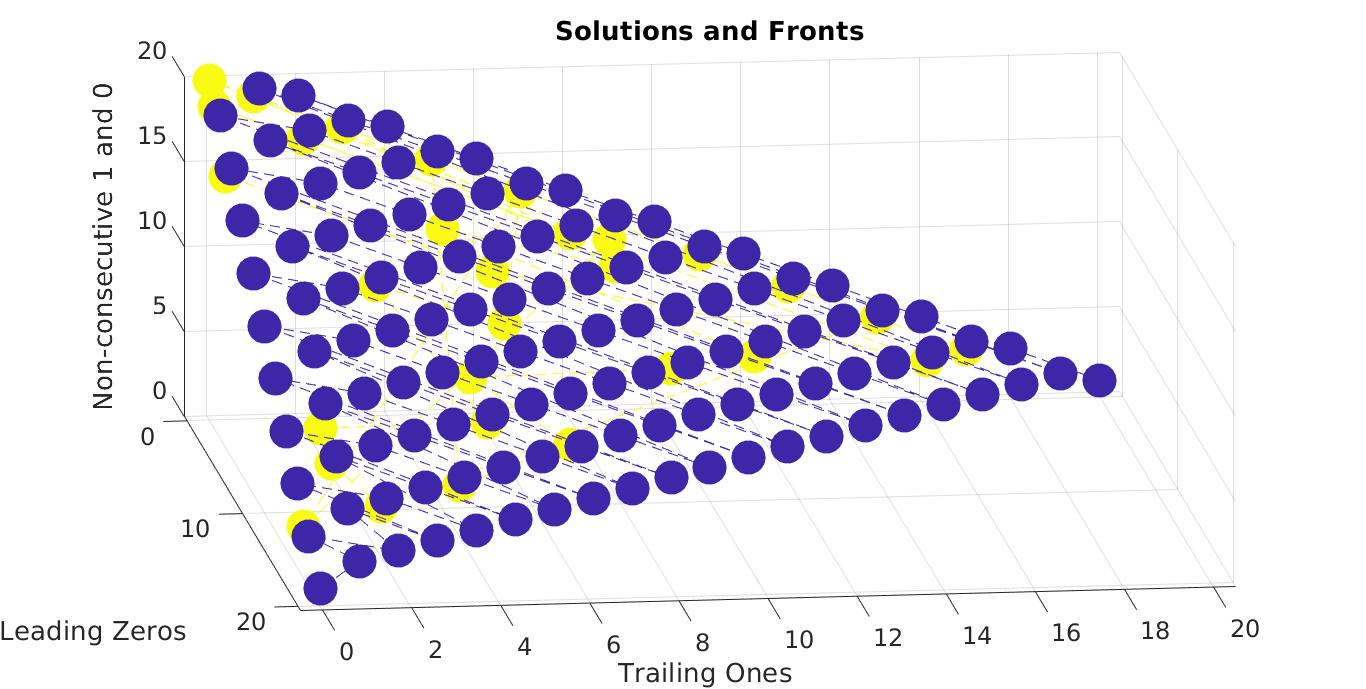
\includegraphics[width=1.0\linewidth]{3dextraQuestion.jpg}
            \caption{NSGA2 algorithm with 3 fitness (leading zeros, trailing ones and non-consecutive 1 and 0) ran for 200 gen with 150 pop for bitstring of size 20.}\label{fig:3dplot}
        \end{figure}
\end{enumerate}


\end{document}














